\section{Đề xuất phát triển}

\subsection{Chiến lược khai phá đặc trưng dựa trên độ trùng lắp}

Ảnh tham khảo truy xuất được từ tác vụ VPR tiềm ẩn rủi ro không đủ độ trùng lắp với ảnh đầu vào, dẫn đến sai sót trong quá trình tính toán tư thế. Để giải quyết vấn đề này, chúng tôi đề xuất một chiến lược khai phá mới dựa trên Multi-Similarity Miner \cite{wang2019multi} nhằm đảm bảo tính trùng lắp đặc trưng trực quan cao giữa các ảnh, nhằm mục đích giúp cho tác vụ RPR thực hiện hồi quy tư thế dễ dàng hơn. 

Cụ thể hơn, chúng tôi xác định một cặp ảnh là được chấp nhận nếu có độ trùng lắp frustum cao hơn một ngưỡng nhất định, tức giữa cặp ảnh chia sẻ nhiều đặc điểm chung hơn, nhằm đảm bảo quy trình dự đoán tư thế chuẩn xác hơn. Để đảm bảo độ vững chắc của mô hình không bị tác động, chúng tôi sử dụng cơ chế trùng lắp camera frustum song phương từ \cite{9008579}, được tính bằng tổng độ trùng lắp frustum từ một ảnh đến ảnh còn lại và ngược lại.

\begin{figure}[H]
  \centering
  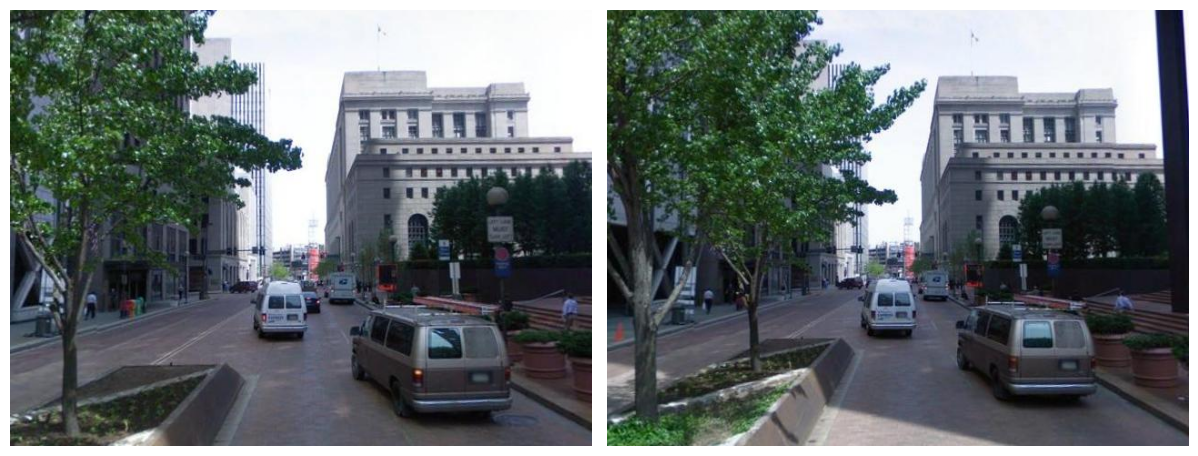
\includegraphics[width=\textwidth]{pics/Chapter3/highoverlap.png}
  \caption[Cặp ảnh có độ overlap cao]{Cặp ảnh được chấp nhận - có độ trùng lắp cao}
\end{figure}

\begin{figure}[H]
  \centering
  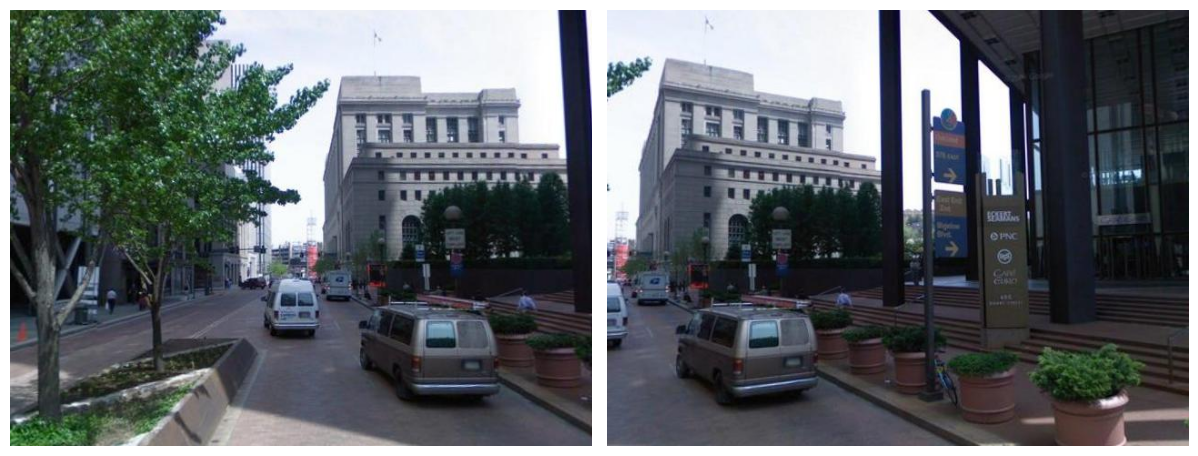
\includegraphics[width=\textwidth]{pics/Chapter3/lowoverlap.png}
  \caption[Cặp ảnh có độ overlap thấp]{Cặp ảnh không được chấp nhận - có độ trùng lắp thấp}
\end{figure}

Tuy nhiên, độ trùng lắp cao vẫn có thể xuất hiện trong trường hợp các ảnh được chụp ở hai góc độ hoàn toàn ngược nhau, gây nên khó khăn và sai lệch trong quá trình dự đoán tư thế tuyệt đối do góc quay khác biệt quá lớn. Để giải quyết vấn đề này, chúng tôi đặt ra điều kiện khác biệt hướng nhìn làm một tiêu chuẩn phụ trong việc chấp nhận các cặp ảnh. Cụ thể hơn, các cặp ảnh không được phép có hướng nhìn lệch nhau quá một tiêu chuẩn nhất định mà chúng tôi đặt ra.

\subsubsection*{Độ trùng lắp Frustum}

Độ trùng lắp frustum giữa hai ảnh có thể được định nghĩa là tổng tỷ lệ các điểm ảnh thuộc ảnh thứ nhất nằm trong vùng tầm nhìn khi chiếu lên hệ tọa độ camera thứ hai, và ngược lại. Độ trùng lắp này được tính toán bằng cách trước hết chiếu các điểm ảnh từ hình ảnh gốc vào không gian 3D thông qua việc tận dụng độ sâu được ước lượng. Sau đó, các điểm ảnh này được chiếu vào hệ tọa độ của hình ảnh thứ hai bằng cách tận dụng thông tin vị trí và góc quay của chúng.

Đầu tiên, một ma trận các điểm ảnh với kích thước 10x10 được chiếu vào hệ tọa độ thực, sau đó lại được chiếu lại vào hệ tọa độ camera thứ hai. Phép chiếu có thể được công thức hóa như sau:
$$
W = R_1\cdot \left[(K_1^{-1} \cdot P_1)*D_1(P_1)\right] + t_1
$$

$$
P_2 = K_2 \cdot\left[R_2^{T} \cdot (W - t_2)\right]
$$
với $P_i$ là vị trí điểm ảnh trong camera $i$, $K_i$ là ma trận intrinsics, $R_i$ và $t_i$ là độ lệch góc quay và vị trí từ hệ tọa độ camera sang hệ tọa độ thực với $R$ là vector góc quay thu được từ quaternion tương ứng, và $D_i(P)$ là ước lượng độ sâu theo đơn vị khoảng cách của điểm ảnh $P$.

\subsubsection*{Khác biệt hướng nhìn}

Để kiểm soát cách biệt góc quay giữa hai ảnh, chúng tôi đo cách biệt về hướng nhìn giữa chúng. Độ lệch góc quay camera $\alpha$ giữa hai camera có thể được định nghĩa như sau:

$$
\alpha = arccos\left(\frac{trace(R_1^T \cdot R_2 - 1)}{2} \right) / \pi * 180
$$

với $\alpha$ mang đơn vị độ.

\subsubsection*{Hàm Loss}

Hàm loss của chúng tôi được tính toán bằng tổng có trọng số giữa hai hàm loss với một biến số 'Control Rate' - tỷ lệ kiểm soát:
$$
L = \beta * L_{Miner} + (1-\beta)*L_{Control}
$$
với $L_{Control}$ là hàm Multi-Similarity Loss từ bài báo Multi-Similarity Miner và $L_{Miner}$ là hàm Multi-Similarity Loss nhận đầu ra từ chiến lược khai phá frustum mới của chúng tôi. 